\documentclass[11pt,a4paper]{beamer}
\usepackage[ngerman]{babel}
\usepackage[T1]{fontenc}
\usepackage[utf8]{inputenc}
\usepackage{amsmath}
\usepackage{amsfonts}
\usepackage{amssymb}
\usepackage[normalem]{ulem}

\usepackage{listings}
\usepackage{color}

\definecolor{dkgreen}{rgb}{0,0.6,0}
\definecolor{gray}{rgb}{0.5,0.5,0.5}
\definecolor{mauve}{rgb}{0.58,0,0.82}

\lstset{frame=tb,
  language=Java,
  aboveskip=3mm,
  belowskip=3mm,
  showstringspaces=false,
  columns=flexible,
  basicstyle={\small\ttfamily},
  numbers=none,
  numberstyle=\tiny\color{gray},
  keywordstyle=\color{blue},
  commentstyle=\color{dkgreen},
  stringstyle=\color{mauve},
  breaklines=true,
  breakatwhitespace=true
  tabsize=3
}

\usepackage{tikz}
\usepackage{gantt}
\usepackage{pgf-umlcd}

% to cross out text
\usepackage{ulem}

\usetheme{Berlin}
\author{Julian Baumann, Xenia Kühling, Sebastian Ruder}
\title{Koreferenzresolution mit BART}
\subtitle{Abschlusssvortrag zum Softwareprojekt im Sommersemester 2014}
\date{22. Juli 2014}

\begin{document}
\maketitle

\section{Einführung}
\begin{frame}{Inhalt}
\tableofcontents
\end{frame}

\begin{frame}{Aufgabe revisited}
Grundsätzlich: System für Koreferenzresolution
\begin{itemize}
\item Vorher: BART
\item Nachher: BART mit neuem Ansatz
\begin{itemize}
\item Implementierung von vorwiegend regelbasiertem System der Stanford-NLP-Gruppe
\item Bestes Ergebnis bei CoNLL-2011 shared task
\item 10 zu implementierende Sieves, erstmal nur für Deutsch
\end{itemize}
\end{itemize}
\end{frame}


\begin{frame}{Aufbau des Stanford Systems revisited}
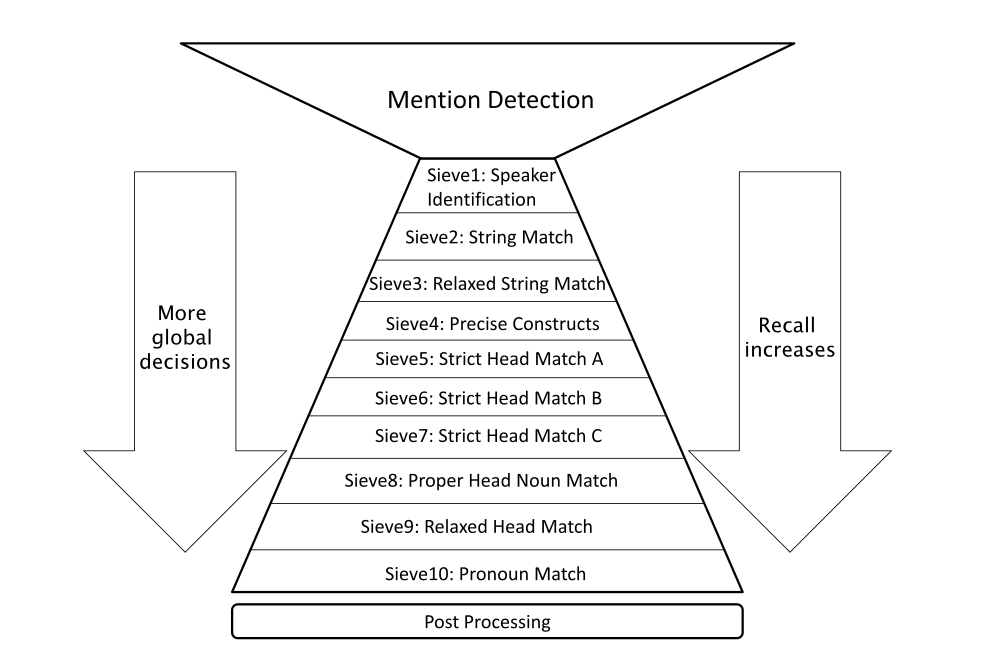
\includegraphics[scale=0.29]{stanford.png}
\end{frame}


\section{Softwarespezifikation}

\begin{frame}
\frametitle{Softwarespezifikation}

\begin{itemize}

	\item Datenformate
		\begin{itemize}
		\item MMAX2, Java, .config, \textcolor{green}{.py, CoNLL}
	\end{itemize}
	\item BART-Version: Klon von Yannicks bitbucket \textit{repository} (\url{https://bitbucket.org/yannick/bart}); Stand 05.05.14 
	\item Korpora
	\begin{itemize}
		\item TüBA-D/Z 2008 MMAX2 (Deutsch)
		\item \sout{Penn Treebank (Englisch)} \textcolor{green}{OntoNotes}
		\item \sout{Turin University Treebank/ISST (Italienisch)}
	\end{itemize}
	\item Programmierumgebung
	\begin{itemize}
		\item Eclipse 4.3.2 mit IvyDE (\textit{dependency management}) s
	\end{itemize}

\end{itemize}

\end{frame}

\begin{frame}{Organisation} 
	\begin{itemize}
	\item Versionskontrolle: Github mit Egit
	\item Einmal wöchentlich regelmäßiges Treffen, sonst nach Absprache
	\item GoogleDocs Dokument um Besprochenes und Ziele/Aufgaben festzuhalten
	\item Skype/WhatsApp Gruppe
	\item \textbf{Email!!!}
	
	\end{itemize}
\end{frame}
\section{Module}

\begin{frame}
\frametitle{Endgültige Architektur}

\begin{tikzpicture}
  \begin{interface}[text width = 3cm]{corefResolver}{-1,5}  	
    \operation{decodeDocument (List<Mention> mentions, Map<Mention,Mention> antecedents : DisjointSet<Mention>)}
  \end{interface}
  
  \begin{class}[text width = 3cm]{SieveDecoder}{-1,0}    
    \implement{corefResolver}
    \attribute{sieves : List<Sieve>}
  \end{class}
  
   \begin{abstractclass}{Sieve}{5,5}
    \operation{runSieve(Mention mention, Mention potAnt) : int}
  \end{abstractclass}
  
   \begin{class}[text width = 2.5cm]{concreteSieve1}{3,0}
    \inherit{Sieve}
  \end{class}
  
   \begin{class}[text width = 2.5cm]{concreteSieve2}{7,0}
    \inherit{Sieve}
  \end{class}
  

\end{tikzpicture}
\end{frame}

\begin{frame}
\frametitle{Discourse Entity}

\begin{tikzpicture}
  \begin{class}[text width =10cm] {DiscourseEntity}{0,0}
  	\attribute{mentions : set<Mention>}
  	\attribute{\uline{nextID} : int}
  	\attribute{discourseID : ID}
    \attribute{genders : set<Gender>}
    \attribute{numbers : set<G}
	\attribute{words : set<String>}
	\attribute{heads : set<String>}
	\attribute{firstMention : Mention}
	\attribute{representativeMention : Mention}
    \operation{DiscourseEntity(Mention m)}
    
    \operation{mergeEntities(Mention m) : void}
    \operation{getMostRepresentativeMention() : void}
  \end{class}
\end{tikzpicture}

\end{frame}

\begin{frame}[fragile]
\begin{lstlisting}
public DisjointSet<Mention> decodeDocument(List<Mention> mentions,Map<Mention, Mention> antecedents) {   		
    Sieve sieve;        
    for (int walk_through = 1; walk_through < 11; walk_through++) {       	
        	//all Mentions or only first Mentions  
        List<Mention> mentionsToResolve;  
        sieve = _factory.createSieve(walk_through, mentions);
        for (int i = 0; i < mentionsToResolve.size(); i++) {		    	
            int ante_idx = sieve.runSieve(mentions.get(i));
            if (ante_idx != -1) {
                //merge Entities
        }        _
	    return mention_clusters;
	}
\end{lstlisting}

\end{frame}

\begin{frame}[fragile]
\frametitle{Sieve}
\begin{lstlisting}
	public abstract class Sieve {

	protected String name; // name of sub class	
	protected List<Mention> mentions;
	 
	abstract int runSieve(Mention mention);
	
	public String getName() {
	    return this.name;
		
	//various helping Methods
	}
\end{lstlisting}
\end{frame}

\begin{frame}[fragile]
\frametitle{PreciseConstructsSieve}
\begin{lstlisting}
int runSieve(Mention mention) {
    PairInstance pair;
    int mention_idx = mentions.indexOf(mention);
    int ante_idx = -1;
		
    for (int idx = 0; idx < mention_idx; idx++) {			
        pair = new PairInstance(mention, mentions.get(idx));
        if (isRelativePronoun(pair) || isAcronym(pair) || isDemonym(pair) || isRoleAppositive(pair)){            
            ante_idx = idx;
        }
    }
    return ante_idx;
}
\end{lstlisting}
\end{frame}

\begin{frame}[fragile]
\frametitle{isRoleAppositive}
\begin{lstlisting}
//[[actress] Rebecca Schaeffer]

boolean isRoleAppositive(PairInstance pair) {
    Mention mention = pair.getAnaphor();
    Mention antecedent = pair.getAntecedent();
    
    if (mention.getProperName() && // check if person
        isAnimate(antecedent) && // check if animate
        !isNeutral(antecedent) && // check if neutral
        mention.embeds(antecedent)) { // check if antecedent is contained in mention							
            return true;
		}
		return false;
	}
\end{lstlisting}
\end{frame}

\begin{frame}{Repository-Struktur}
\begin{figure}
\begin{center}
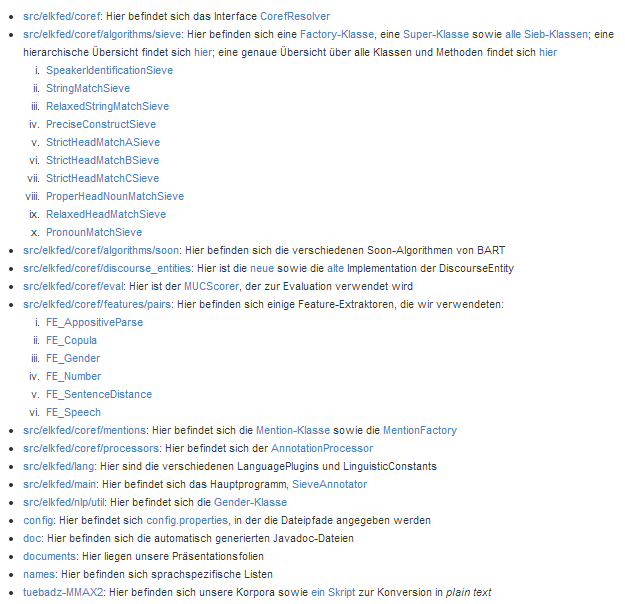
\includegraphics[width=7cm]{repository_structure.png}
\caption{Struktur des \textit{repository}}
\label{fig:repository}
\end{center}
\end{figure}
\end{frame}

\section{Demonstration}
\begin{frame}{Demo}
Man sehe und staune! :)
\end{frame}


\section{Evaluation}
\begin{frame}{Insgesamt}
\begin{table}[h]
\begin{tabular}{llll}
                            & \textbf{Recall} & \textbf{Precision} & \textbf{F-Score} \\
SpeakerIdentification       & 0.05            & 0.360              & 0.010            \\
\textbf{+StringMatch}       & 0.138           & 0.748              & 0.232            \\
+RelaxedStringMatch         & 0.149           & 0.740              & 0.248            \\
\textbf{+PreciseConstructs} & 0.200           & \textbf{0.759}     & 0.317            \\
\textbf{+StrictHeadMatchA}  & 0.282           & 0.714              & 0.404            \\
\textbf{+StrictHeadMatchB}  & 0.334           & 0.672              & 0.446            \\
+StrictHeadMatchC           & 0.344           & 0.661              & 0.453            \\
+ProperHeadNounMatch        & 0.348           & \textbf{0.663}     & 0.456            \\
+RelaxedHeadMatch           & 0.371           & 0.669              & 0.478            \\
\textbf{+PronounMatch}      & 0.496           & 0.630              & \textbf{0.555}       
\end{tabular}
\caption{MUC-Score, TueBa-D/Z 1-100}
\end{table}
\end{frame}

\begin{frame}{perSieve}
\begin{table}[h]
\begin{tabular}{lcc}
                           & \textbf{Total Mentions} & \textbf{correct Links} \\
                          &\textbf{Linked}			&\\
SpeakerIdentificationSieve & 25                             & 9                      \\
StringMatchSieve           & 312                            & 243   					\\
RelaxedStringMatchSieve    & 37                             & 24                     \\
PreciseConstructSieve      & 115                            & 94                     \\
StrictHeadMatchASieve      & 243                            & 151                    \\
StrictHeadMatchBSieve      & 197                            & 99                     \\
StrictHeadMatchCSieve      & 53                             & 24                     \\
RelaxedHeadMatchSieve      & 68                             & 52                     \\
ProperHeadNounMatchSieve   & 8                              & 5                      \\
PronounMatchSieve          & 425                            & 170                    \\
\end{tabular}
\caption{MUC-Score, TueBa-D/Z 1-100}
\end{table}
\end{frame}


\begin{frame}{Vergleich mit Stanford Sieves + BART, conll 2011 shared task, Englisch}
Stanford Sieves Englisch vs. BART vs. unser BART\\

s. http://conll.cemantix.org/2011/
\end{frame}

\begin{frame}{Direkter Vergleich mit BART Deutsch}

Beispiel BART

\begin{tabular}{|c|c|c|c|}
\hline 
ID & RECALL & PRECISION & F1 \\ 
\hline 
export001 & 0.508 & 0.642 & 0.567 \\ 
\hline 
export002 & 0.467 & 0.778   & 0.584 \\ 
\hline 
export003 & 0.101 & 0.250 & 0.143 \\ 
\hline 
SCORER MUC-TOTAL & 0.457 & 0.637   & 0.532 \\
\hline

\end{tabular} 
\end{frame}

\begin{frame}{Vergleich der einzelnen Sieves}
Welches Sieve macht wie viel, eventuell Vergleich mit Stanford Sieves (welche Sieves sind bei uns toll, welche bei Stanford?)

\end{frame}
  

\section{Zeitplan}

\begin{frame}

    \begin{gantt}{10}{9}
    \begin{ganttitle}
      \titleelement{Mai}{1}
      \titleelement{Juni}{4}
      \titleelement{Juli}{4}
    \end{ganttitle}
    \begin{ganttitle}
      \titleelement{27.05.}{1}
      \titleelement{03.06.}{1}
      \titleelement{10.06.}{1}
      \titleelement{17.06.}{1}
      \titleelement{24.06.}{1}      
      \titleelement{01.07.}{1}
      \titleelement{08.07.}{1}
      \titleelement{15.07.}{1}
      \titleelement{22.07.}{1}
    \end{ganttitle}
    \ganttbar{Pipeline läuft}{0}{2}
    \ganttmilestone[color=blue]{1. \textit{Sieve} läuft}{2}
    \ganttbar{\textit{Sieves} einfügen}{2}{3}
    \ganttmilestone[color=blue]{\textit{Sieves} laufen}{5}
    \ganttbar{Evaluation}{5}{3}
    \ganttbar[color=blue]{Bugfixes}{2}{6}
    \ganttbar{Präsentation}{7}{1}
    \ganttbar[color=blue]{Dokumentation}{5}{4}
  \end{gantt}
  
\end{frame}

\begin{frame}{\textit{Workload} im Laufe des Softwareprojekts}
\begin{figure}
\begin{center}
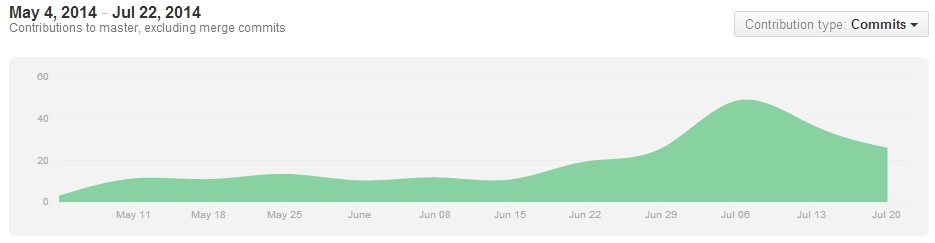
\includegraphics[width=11cm]{contributions_to_master.jpg}
\caption{Commits von 04.05. - 22.07.14}
\label{fig:contributions}
\end{center}
\end{figure}
\end{frame}


\section{Lessons learned}
\begin{frame}{Probleme mit der Technik / dem Korpus}
\begin{itemize}
\item EGit für Eclipse manchmal sehr buggy
\item Konversionsfehler im Korpus $\rightarrow$ falscher Goldstandard
\item parse-Level fehlte anfangs $\rightarrow$ Headfinder funktionierte nicht
\item TüBaD/Z Headfinder hat danach auch noch nicht richtig funktioniert $\rightarrow$ Regel in BART musste geändert werden
\item \texttt{getNumber()} gab stets \texttt{Singular} zurück 
\end{itemize}
$\rightarrow$ intimes Wissen des Systems zur Auflösung von technischen Diskrepanzen vonnöten

\end{frame}

\begin{frame}{Probleme mit BART und dem Stanfordsystem}
\begin{itemize}
\item Stanford-System prinzipiell sprach- und korpusübergreifend anwendbar, aber für Englisch und OntoNotes optimiert\\
$\rightarrow$ Erweiterung des \texttt{GermanLanguagePlugins}, \texttt{GermanLinguisticConstants}
\item Viele Methoden in BART unklar / unzureichend dokumentiert
\item Modulübersicht wäre praktisch gewesen
\item Stanford Code unübersichtlich / verwirrend modularisiert\\$\rightarrow$ wenig Anreiz sich daran zu orientieren
\end{itemize}
$\rightarrow$ Einarbeitung in ein fremdes System ist ein beträchtlicher, kontinuierlicher Zeitaufwand\\
$\rightarrow$ Ein Ansprechpartner, der in das System einführen und bei systemspezifischen Fragen Hilfestellung geben kann, ist sehr wertvoll\\
$\rightarrow$ Nachvollziehbare Dokumentation daher umso wichtiger!
\end{frame}

\section{Ausblick}
\begin{frame}{TO DO bis Abgabeschluss}
\begin{itemize}
\item Dokumentation finalisieren; Abschlussbericht verfassen
\item Sieves verfeinern, im Speziellen \texttt{PronounMatch}, \texttt{StrictHeadMatch}, \texttt{SpeakerIdentification}
\item Auf OntoNotes-Korpus evaluieren
\item TüBa-D/Z-Output in CoNLL-Format, mit CoNLL-Scorer scoren und mit SemEval-Systemen vergleichen
\end{itemize}
\end{frame}

\begin{frame}{Ausblick}
\begin{itemize}
\item System für das Englische, Italienische und andere Sprachen optimieren
\item neue, fürs Deutsche optimierte Sieves verwenden
\item aktuelle Sieves weiter verbessern
\item Dependenzen in BART bereinigen, relevante Komponenten abgrenzen, ausführlich dokumentieren
\item Ähnlichkeit basierend auf GermaNet als Feature verwenden
\item Koreferenzen, die auf Weltwissen basieren, erfordern fortgeschrittene Wissensdatenbanken, z.B.:\\
  \begin{itemize}
  \item \textit{Mention:} “die organisierte Totmacherei, die heute ‘humanitäre Invervention’ heißt”; \textit{Antezedent:} “den Krieg”\\
  \item \textit{Mention:} “das Werk”; \textit{Antezedent:} “ein verspätetes Geburtstagsgedicht für den Dieter von Modern Talking”\\
  \end{itemize}
\end{itemize}
\end{frame}


%\section{Quellen}
%\begin{frame}{Quellen}
%\nocite{*}
%\bibliographystyle{abbrv}
%\bibliography{lit}
%\end{frame}

\end{document}
